\documentclass{beamer}
\usetheme{Madrid}

\usepackage{cmap}
\usepackage[T2A]{fontenc}
\usepackage[russian,english]{babel}
\usepackage[utf8]{inputenc}
\usepackage{amsmath, amssymb}
\usepackage{minted}
\usepackage{hologo}

\usepackage{algorithm2e}
\usepackage{algorithmic}
\usepackage{float}

% \newtcbox{\mybox}{blank, on line, opacitytext=0.5}

\title[Ускорение обучения языковых моделей]{Методы предобработки текстовых данных для ускорения обучения языковых моделей}

\author[Сурков М.К.]{Сурков Максим Константинович\\
 	{\footnotesize Научный руководитель: Ямщиков Иван Павлович}
}
\institute[НИУ ВШЭ СПБ]{Санкт-Петербургская школа физико-математических и компьютерных наук \\ НИУ ВШЭ СПБ}
\date{17 марта 2021 г.}

\begin{document}

\frame{\titlepage}

\begin{frame}
\frametitle{Обработка естественного языка в реальной жизни}
\begin{columns}
	\column{0.5\textwidth}
	\begin{itemize}
		\item социальные сети
		\item электронная почта
		\item службы доставки
		\item голосовые помощники
		\item переводчики
		\item чат боты
	\end{itemize}
	\column{0.5\textwidth}
	
\includegraphics[scale=0.2]{nlp_real_life.png}
\end{columns}
\end{frame}

\begin{frame}
\frametitle{Задачи обработки естественного языка}
\begin{enumerate}
	\item классификация последовательностей
		\begin{itemize}
			\item спам
			\item грубая речь\footnote[1]{G. H. Paetzold et al., SemEval'19 Task 5: Hate Speech Identification with RNN.}
		\end{itemize}
	\item генерация выходной последовательности из исходной
		\begin{itemize}
			\item машинный перевод
			\item ответы на вопросы
		\end{itemize}
	\item выделение информации из последовательностей
		\begin{itemize}
			\item выделение именованных сущностей\footnote[2]{Vikas Yadav et al., SemEval'19 Task 12: Deep-Affix Named Entity Recognition of Geolocation Entities. ACL'19}
		\end{itemize}
\end{enumerate}

\end{frame}

\begin{frame}
	\frametitle{Современные методы решения задач обработки естественного языка}
	\begin{enumerate}
		\item Механизм внимания\footnote[1]{Ashish Vaswani et al., Attention Is All You Need, 2017}
		\item {\bf BERT} (Google)\footnote[2]{Jacob Devlin et al., BERT: Pre-training of Deep Bidirectional Transformers for Language Understanding, 2019}
		\item GPT-3 (OpenAI)\footnote[3]{Tom B. Brown et al., Language Models are Few-Shot Learners, 2020}
	\end{enumerate}
\end{frame}

\begin{frame}
	\frametitle{BERT. Использование}
	\begin{center}
		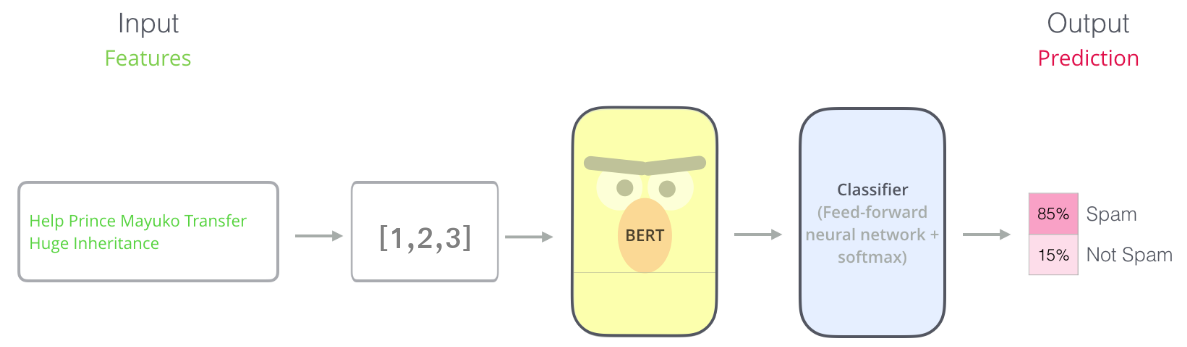
\includegraphics[scale=0.35]{bert_usage.png}
	\end{center}
\end{frame}

\begin{frame}
	\frametitle{BERT. Обучение}
	\begin{center}
		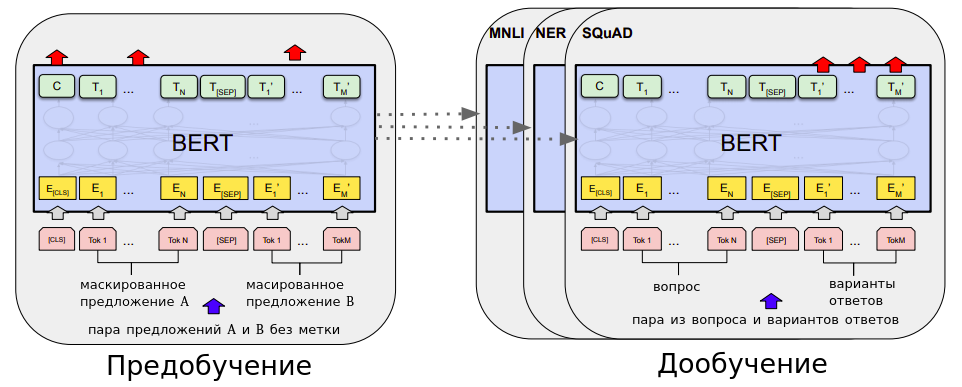
\includegraphics[scale=0.35]{bert_train.png}
	\end{center}
\end{frame}

\begin{frame}
	\frametitle{BERT. Требуемые ресурсы}
	\begin{itemize}
		\item количество параметров: $110M - 340M$
		\item время на предобучение: от 2-4 дней до 1-2 недель\footnote[1]{При использовании 1x-4x GPU Nvidia Tesla V100 32Gb}
		\begin{itemize}
			\item мировой рекорд: 47 минут на {\bf 1472} V100 GPU\footnote[2]{https://developer.nvidia.com/blog/training-bert-with-gpus}
		\end{itemize}
		\item время на дообучение: 1-2 дня
		\item размеры данных:
			\begin{table}
				\begin{tabular}{l|c}
					Датасет & Размер \\
					\hline\hline
					Wikipedia & 3-600M \\
					HND & 600k-2M \\
					s140 & 1.6M \\
					IWSLT & 200-230k \\
					QQP & 364k \\
					MNLI & 393k \\
				\end{tabular}
			\end{table}
	\end{itemize}
\end{frame}

\begin{frame}
	\frametitle{BERT. Существующие методы оптимизации}
	\begin{itemize}
		\item квантизация\footnote[1]{Sheng Shen et al., Q-BERT: Hessian Based Ultra Low Precision Quantization of BERT, 2019}
		\item дистилляция\footnote[2]{Victor Sanh et al., DistilBERT, a distilled version of BERT: smaller, faster, cheaper and lighter, 2020}
		\item прунинг\footnote[3]{Hassan Sajjad et al., Poor Man’s BERT: Smaller and Faster Transformer Models, 2020}
	\end{itemize}
\end{frame}

\begin{frame}
	\frametitle{Обучение с расписанием. Начало}
	
	\begin{center}
		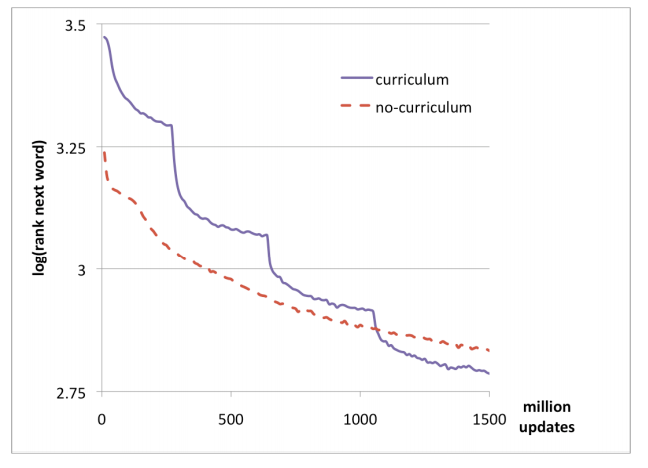
\includegraphics[scale=0.4]{bengio_exp1}
	\end{center}
	
	\let\thefootnote\relax\footnotetext{Y. Bengio et al., Curriculum learning, 2009}
\end{frame}

\begin{frame}
	\frametitle{Обучение с расписанием. Применение}
	\begin{itemize}
		\item компьютерное зрение\footnote[1]{Guy Hacohen, Daphna Weinshall, On The Power of Curriculum Learning in Training Deep Networks, 2019}

		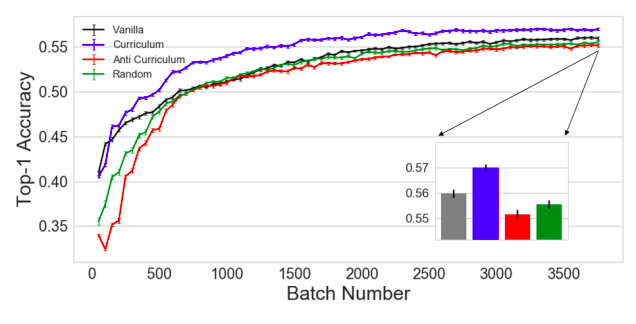
\includegraphics[scale=0.3]{curriculum_learning_cv}
		
		\item обучение с подкреплением\footnote[2]{Sanmit Narvekar et al., Curriculum Learning for Reinforcement Learning Domains: A Framework and Survey, 2020}
		
		\item глубокое обучение\footnote[3]{Mermer et al., Scalable Curriculum Learning for Artificial Neural Networks, 2017}
	\end{itemize}
\end{frame}

\begin{frame}
	\frametitle{Обучение с расписанием в обработке языка}		\let\thefootnote\relax\footnotetext{E. A. Platanios et al., Competence-based Curriculum Learning for Neural Machine Translation, ACL'19}
	\begin{itemize}
		\item Задача: машинный первод
		\item Модель: BERT, LSTM
		\item Датасеты: IWSLT'15, IWSLT'16, WMT'16
		\item Алгоритм:
			\begin{columns}
				\column{0.5\textwidth}
					\begin{enumerate}
						\item сортируем тексты по сложности (длина, логарифм веротности правдоподобия)
						\item в течение $T$ шагов (рассмотрим шаг $t$)
						\begin{itemize}
							\item считаем $c(t) \in [0, 1]$
							\item строим батч из $c(t)$ {\bf первых} текстов корпуса
							\item шаг обучения
						\end{itemize}
					\end{enumerate}
				\column{0.5\textwidth}
				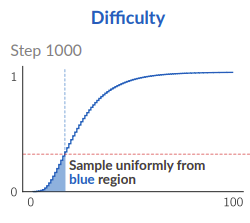
\includegraphics[scale=0.6]{acl19_algo.png}
			\end{columns}
	\end{itemize}
\end{frame}

\begin{frame}
	\frametitle{Обучение с расписанием в обработке языка}
	\begin{center}
		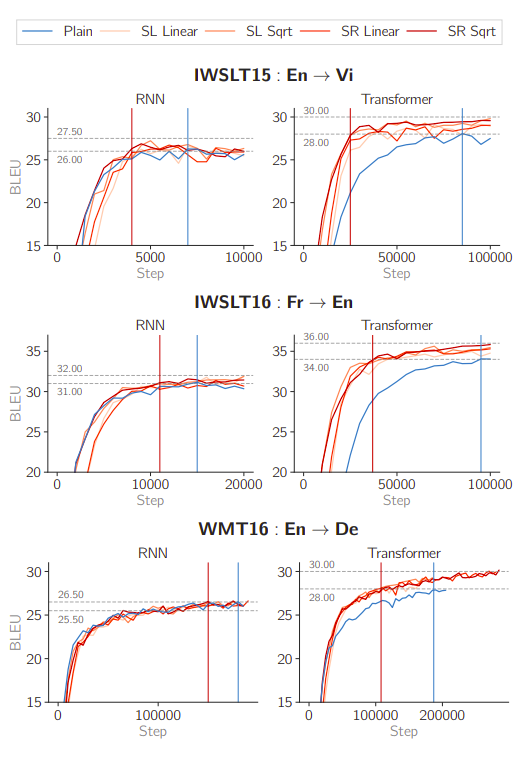
\includegraphics[scale=0.3]{acl19_results}
	\end{center}
\end{frame}

\begin{frame}
	\frametitle{Обучение с расписанием в обработке языка}		\let\thefootnote\relax\footnotetext{Benfeng Xu et al., Curriculum Learning for Natural Language Understanding, ACL'20}
	\begin{itemize}
		\item Задача: классификация
		\item BERT
		\item Датасеты: SQuAD 2.0, NewsQA, GLUE
		\item Алгоритм: в течение $T$ шагов
			\begin{center}
				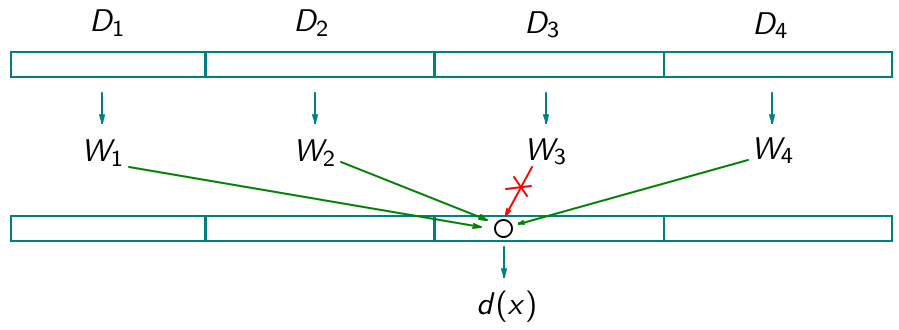
\includegraphics[scale=0.45]{acl20_algo_difficulty}
			\end{center}
	\end{itemize}
\end{frame}

\begin{frame}
	\frametitle{Обучение с расписанием в обработке языка}
	\begin{center}
		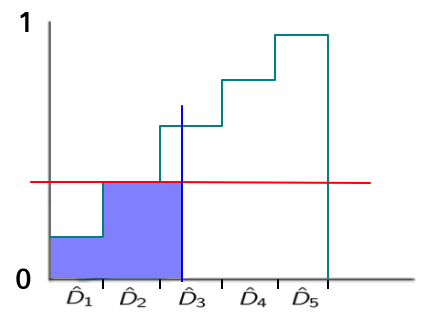
\includegraphics[scale=0.6]{acl20_algo_sampler}
	\end{center}
\end{frame}

\begin{frame}
	\frametitle{Обучение с расписанием в обработке языка}
	\begin{center}
		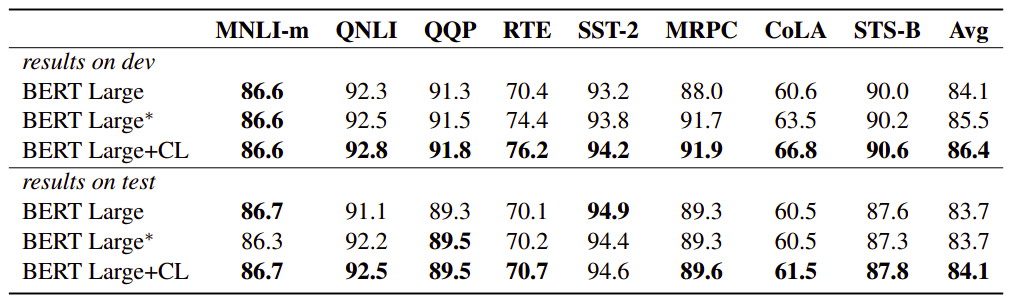
\includegraphics[scale=0.3]{acl20_results}
	\end{center}

	\begin{center}
		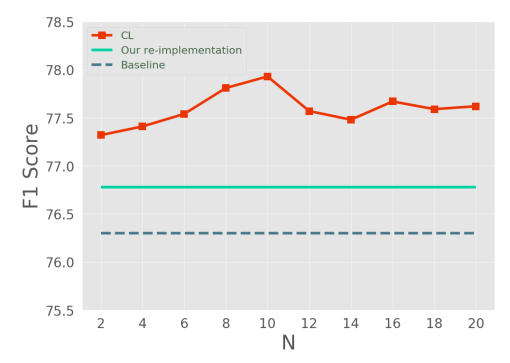
\includegraphics[scale=0.3]{acl20_results2}
	\end{center}

\end{frame}

\begin{frame}
	\frametitle{Обучение с расписанием в обработке языка. Направления для исследований}
	\begin{itemize}
		\item Много важных задач обработки естественного языка с {\bf большими} корпусами тренировочных данных
		\item Решаются с помощью {\bf тяжелых} моделей, которые {\bf долго} учатся
		\item Не иcследованы метрики оценки сложности текста (длина - текущий предел)
		\item Эксперименты проведены только на определенных задачах
			\begin{itemize}
				\item ACL'19 - только задача машинного перевода
				\item ACL'20 - только задача классификации\footnote[1]{Не совсем честное обучение с расписанием; Не ускоряет; Требует еще больших ресурсов}
			\end{itemize}
		\item Не исследовано влияние обучения с расписанием на этапе предобучения
	\end{itemize}
\end{frame}

\begin{frame}
	\frametitle{Цели и задачи}
	{\bf Цель:} ускорить обучение языковой модели BERT с помощью обучения с расписанием за счет метрики оценки сложности текстовых данных на задачах предобучения, классификации и машинного перевода

	{\bf Задачи:}
	\begin{enumerate}
		\item Найти эффективные\footnote[1]{с точки зрения сокрости обучения модели} метрики оценки сложности текста
		\item Реализовать механизм подсчета найденных метрик на больших датасетах
		\item Сравнить найденные метрики с существующими метриками оценки сложности текста
		\item Исследовать влияние найденных метрик на скорость обучения языковой модели BERT
	\end{enumerate}
\end{frame}

\begin{frame}
	\frametitle{Поиск метрик}
	\begin{enumerate}
		\item {\bf длина}, вероятность правдоподобия\footnote[1]{E. A. Platanios et al., Competence-based Curriculum Learning for Neural Machine Translation, ACL'19}
		\item информационный поиск
			\begin{itemize}
				\item {\bf tf-idf}
				\item энтропия, семантическая сложность\footnote[2]{Frans van der Sluis et al., Using Complexity Measures in Information Retrieval, 2010}
			\end{itemize}
		\item средняя частота слова, самое редкое слово в предложении\footnote[3]{Xuan Zhang et al., An Empirical Exploration of Curriculum Learning for Neural Machine Translation, 2018}
		\item число определенных частей речи\footnote[4]{Tom Kocmi, Ondrej Bojar, Curriculum Learning and Minibatch Bucketing in Neural Machine Translation, 2017}
		\item {\bf теория информации}
	\end{enumerate}
\end{frame}

\begin{frame}
	\frametitle{Поиск метрик}
	\let\thefootnote\relax\footnotetext{Nihat Ay et al., A {\bf Unifying }Framework for Complexity Measures of Finite Systems, 2006}
		
	\begin{table}
		\begin{tabular}{c|c}
			\hline
			метрика & формула \\
			\hline
			Multi-information & $\sum\limits_{v\in V}H_p(X_v) - H_p(X_V)$ \\
			\hline
			{\bf Excess Entropy (EE)} & $\left[\sum\limits_{v\in V}H(X_{V\backslash\{v\}})\right] - (N - 1)H(X_V)$ \\
			\hline
			{\bf TSE} & $\sum\limits_{k=1}^{N-1}\frac{k}{N}C^{(k)}(X_V)$, где \\\\
			& $C^{(k)}(X_V) = \frac{N}{k\binom{N}{k}}\sum\limits_{A\subseteq V,|A|=k}H(X_A) - H(X_V)$ \\
			\hline
			Transient information & :( \\
			\hline
		\end{tabular}
	\end{table}

	\[
		V=\{1,\ldots,N\}
	\]
	\[
		X_V = (X_1,\ldots,X_N)
	\]
\end{frame}

\begin{frame}
	\frametitle{Адаптация EE и TSE под задачи обработки языка}
	
	\begin{enumerate}
		\item Образование совместной случайной величины
		\[
			T=(t_1, t_2, \ldots, t_{i-1},t_i,\ldots, t_n)
		\]
		\[
			t_i\rightarrow \xi^i_{t_i} =: \mu_i - \text{бинарная случайная величина}
		\]
		\[
			\downarrow
		\]
		\[
			\xi=(\xi^1_{t_1},\xi^2_{t_2},\ldots,\xi^{i-1}_{t_{i-1}},\xi^i_{t_i},\ldots,\xi^n_{t_n})
		\]
		\item Вычисление энтропии
		\[
			H(\mu) = \sum\limits_{i=1}^{n}H(\mu_i|\mu_1,\mu_2,\ldots,\mu_{i-1}) = \sum\limits_{i=1}^{n}H(\mu_i|\mu_{i-k},\ldots,\mu_{i-1})
		\]
		\item $k=1$
		\[
		H(\mu) = H(\mu_1) + H(\mu_2|\mu_1) + \ldots + H(\mu_i|\mu_{i-1}) + \ldots + H(\mu_n|\mu_{n-1})
		\]
	\end{enumerate}
\end{frame}

\begin{frame}
	\frametitle{Вычисление метрик}
	\begin{enumerate}
		\item длина
		\item tf-idf
			\[\sum\limits_{i=1}^{n}f(X_i)\log\frac{|D|}{\{j:X_i\in X^{(j)}\}}\]
			\begin{itemize}
				\item $x_i \rightarrow$ число текстов, в которых есть $x_i$
			\end{itemize}
		\item энтропия для вычисления EE, TSE
			\begin{itemize}
				\item длина $\rightarrow$ число текстов с такой длиной
				\item $(i, x_i) \rightarrow$ число текстов, где $t_i = x_i$ 
				\item $(x_i)\rightarrow$ число текстов, где $x_i$ является последним токеном
				\item $(i, x_{i-1}, x_i) \rightarrow$ число текстов, где на $(i-1)$-й позиции стоит $x_{i-1}$, а на $i$-й позиции стоит $x_i$
			\end{itemize}
		\item EE,TSE - ?
	\end{enumerate}
\end{frame}

\begin{frame}
	\frametitle{Вычисление EE}
	\[
		EE(X) = \left[\sum\limits_{v\in V}H(X_{V\backslash\{v\}})\right] - (N - 1)H(X_V) = 
	\]
	\[
		\left[\sum\limits_{i=1}^{n}H(\mu_1,\ldots,\mu_{i-1},\mu_{i+1},\ldots,\mu_n)\right] - (n - 1)H(\mu)
	\]
	\begin{itemize}
		\item $\mathcal{O}(n^2)$
		\item $\mathcal{O}(n)$
			\[
				\sum\limits_{i=1}^{n}H(\mu_1,\ldots,\mu_{i-1},\mu_{i+1},\ldots,\mu_n) =\]
			\[ = \sum\limits_{i=1}^{n}H(\mu) - H(\mu_i|\mu_{i-1}) - H(\mu_{i+1}|\mu_i) + H(\mu_{i+1})\]
			\[
				EE(X) = \sum\limits_{i=2}^{n}H(\mu_i) - H(\mu_i|\mu_{i-1})= \sum\limits_{i=2}^{n}I(\mu_{i-1}\colon\mu_i)
			\]
	\end{itemize}
\end{frame}

\begin{frame}
	\frametitle{Вычисление TSE}
	\[
		\sum\limits_{k=1}^{N-1}\frac{k}{N}C^{(k)}(X_V)
	\]
	\[
	 	C^{(k)}(X_V) = \frac{N}{k\binom{N}{k}}\sum\limits_{A\subseteq V,|A|=k}H(X_A) - H(X_V) =
 	\]
 	\[
 		= \frac{N}{k}\left[\frac{1}{\binom{N}{k}}\sum\limits_{A\subseteq V,|A|=k}H(X_A)\right] - H(X_V)
	\]
\end{frame}

\begin{frame}
	\frametitle{Вычисление TSE}
		\[
			\frac{1}{\binom{n}{k}}\sum\limits_{A\subseteq V,|A|=k}H(X_A) =
			\frac{1}{\binom{n}{k}}\sum\limits_{1 \le i_1 < i_2 < \ldots < i_k \le n}H(\mu_{i_1}, \mu_{i_2}, \ldots, \mu_{i_k})
		\]
		\begin{enumerate}
			\item $\mathcal{O^*}(2^n)$
			\item $\mathcal{O}(n^2)$ - динамическое программирование
			\item $\mathcal{O}(n)$
				\[
					\sum\limits_{i=1}^{n}A_iH(\mu_i) + \sum\limits_{i=2}^{n}B_iH(\mu_i|\mu_{i-1})
				\]
				\[
					A_i = \frac{\binom{n-1}{k-1}}{\binom{n}{k}} = \frac{k}{n}
				\]
				\[
					B_i = \frac{\binom{n-2}{k-2}}{\binom{n}{k}} = \frac{k(k-1)}{n(n-1)}
				\]
		\end{enumerate}
\end{frame}

\begin{frame}
	\frametitle{Конфигурация экспериментов}
	\begin{itemize}
		\item датасеты
		\begin{table}
			\begin{tabular}{l|c}
				Датасет & Размер \\
				\hline\hline
				Hyperpartisan News Detection\footnote[1]{SemEval-2019 Task 4} & 600k-2M \\
				sentiment140 & 1.6M \\
			\end{tabular}
		\end{table}
		\item метрика качества модели -- точность
		\item модель BERT-base
		\item метод сравнения метрик сложности текста
			\begin{enumerate}
				\item фиксируем модель
				\item фиксируем датасет
				\item фиксируем семплер
				\item учим модели, используя сравниваемые метрики
				\item анализируем график обучения модели
			\end{enumerate}
	\end{itemize}
\end{frame}

\begin{frame}
	\frametitle{Сравнение метрик}
	Без семплера
	\begin{center}
		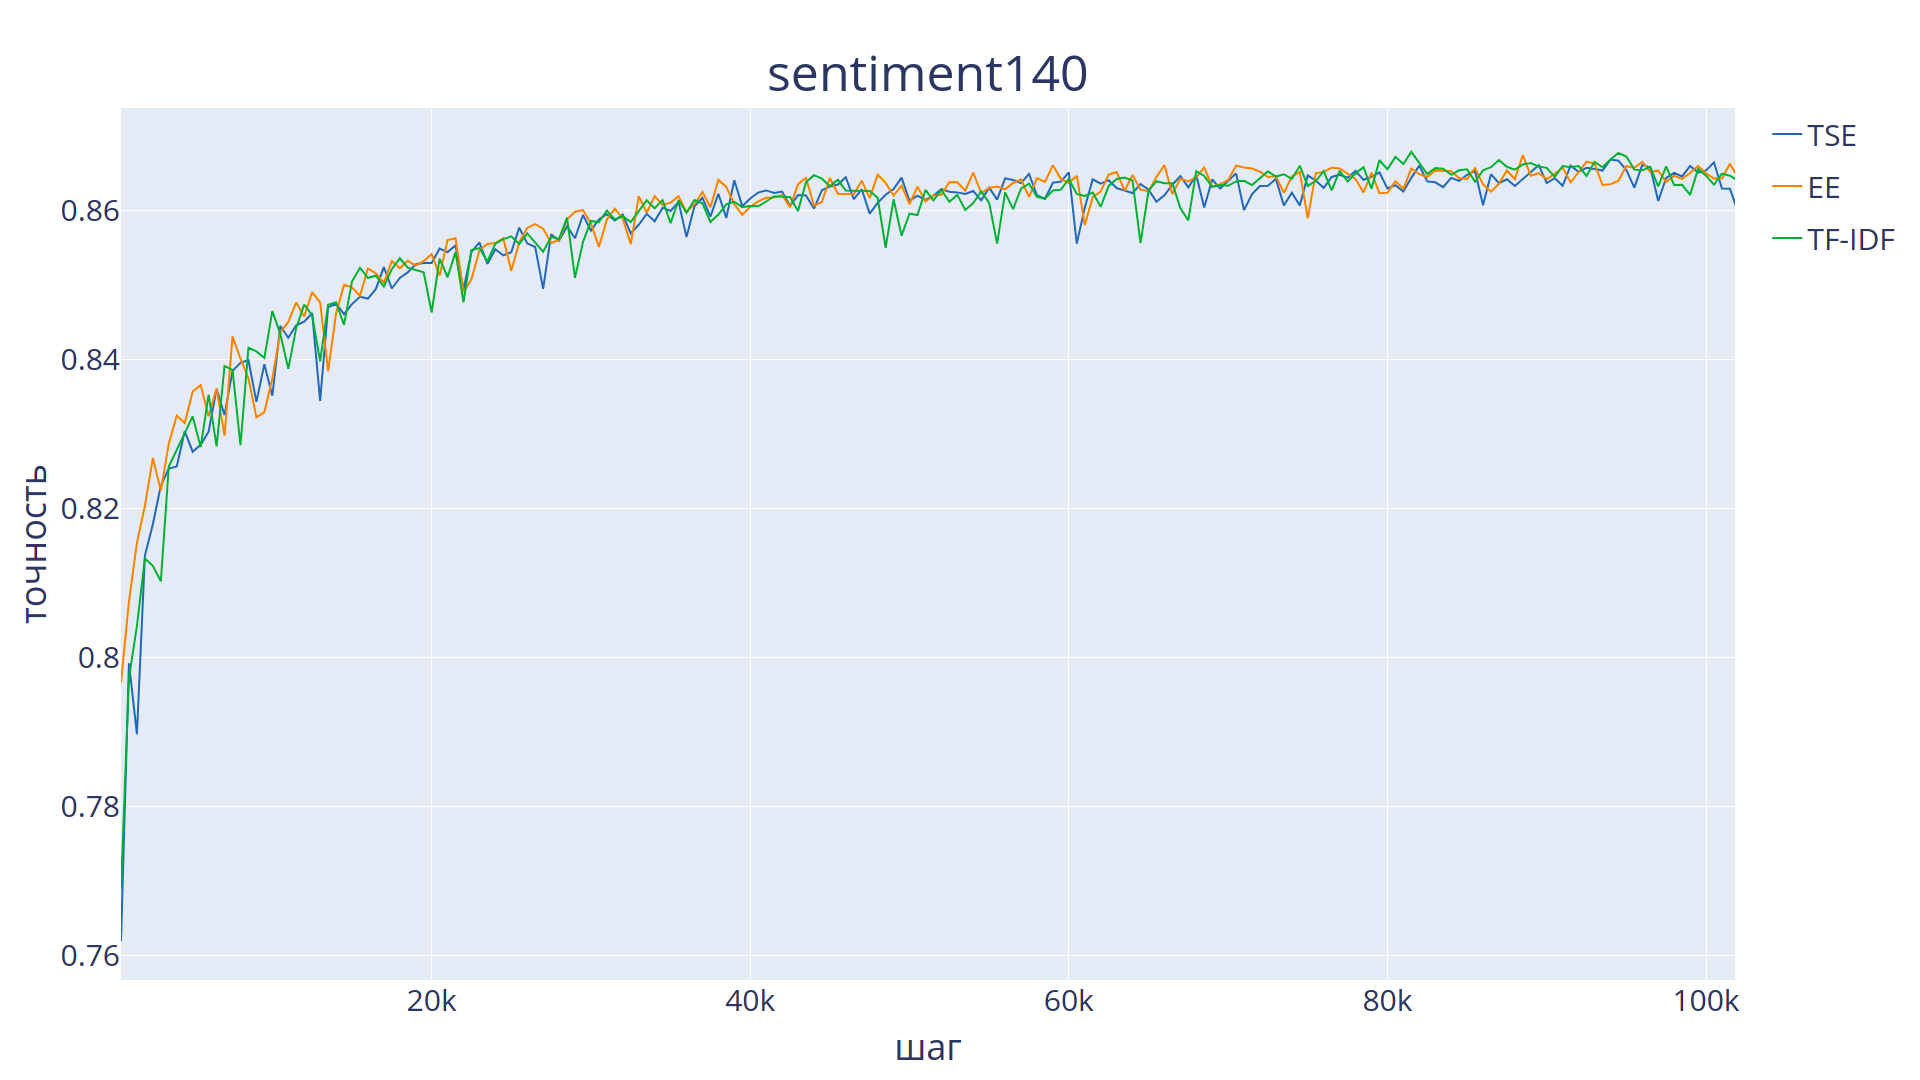
\includegraphics[scale=0.18]{s140_sequential}
	\end{center}
\end{frame}

\begin{frame}
	\frametitle{Сравнение метрик}
	семплер из ACL'19
	\begin{center}
		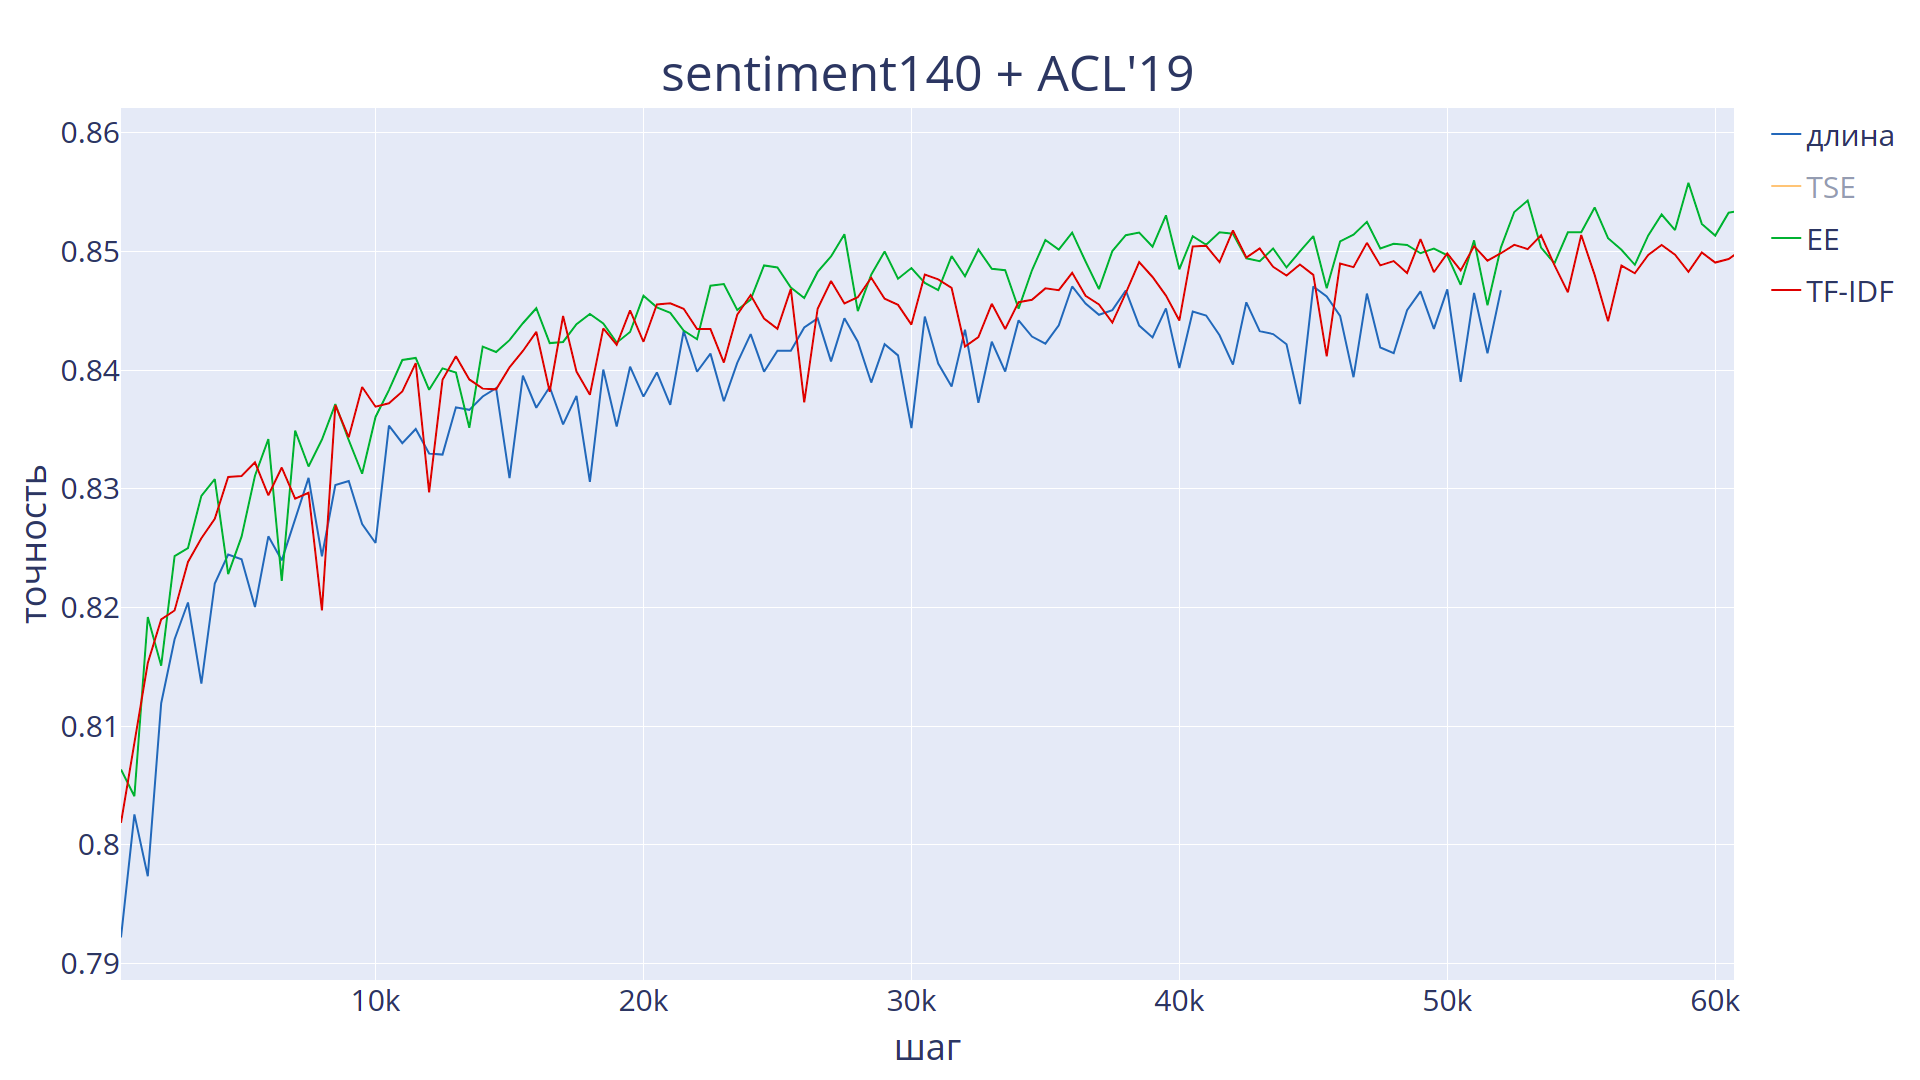
\includegraphics[scale=0.18]{s140_competence_based}
	\end{center}
\end{frame}

\begin{frame}
	\frametitle{Сравнение метрик}
	семплер DB
	\begin{center}
		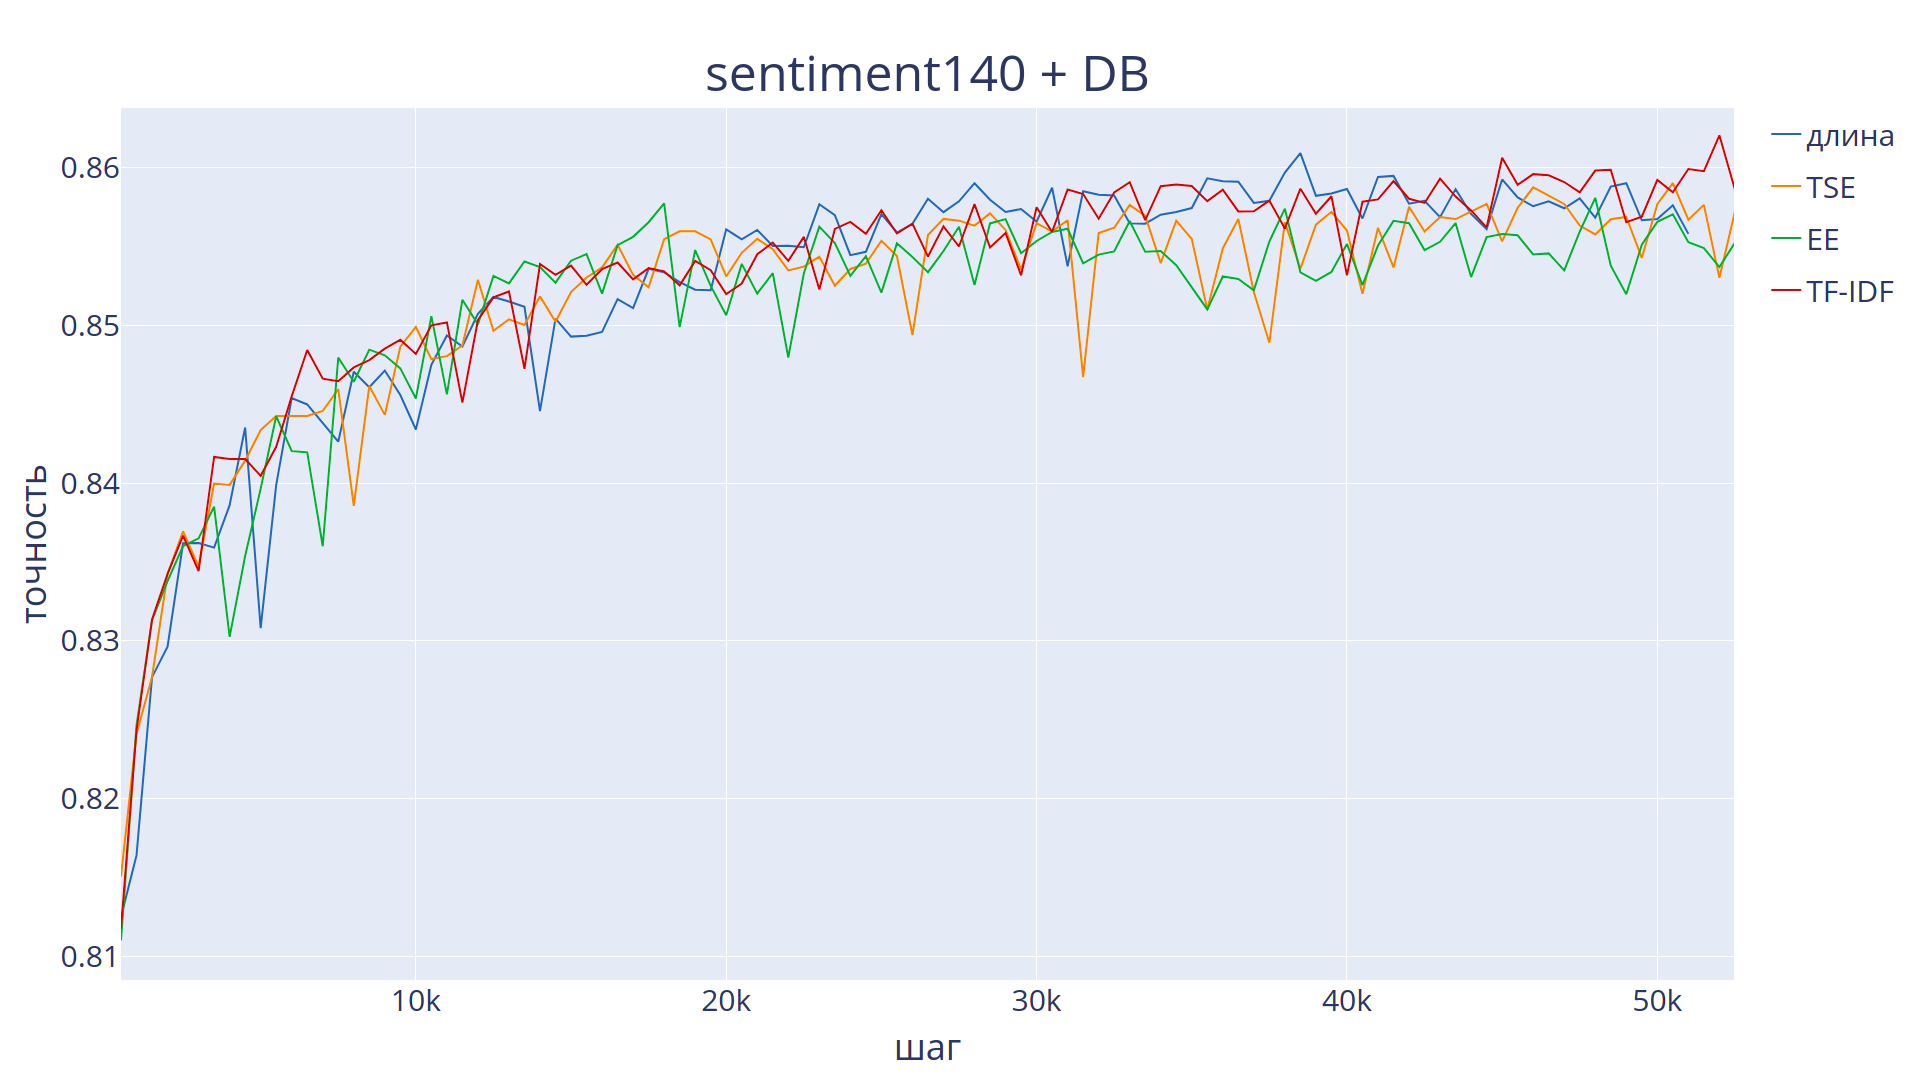
\includegraphics[scale=0.18]{s140_difficulty_based}
	\end{center}
\end{frame}

\begin{frame}
	\frametitle{Сравнение метрик}
	гиперболический семплер
	\begin{center}
		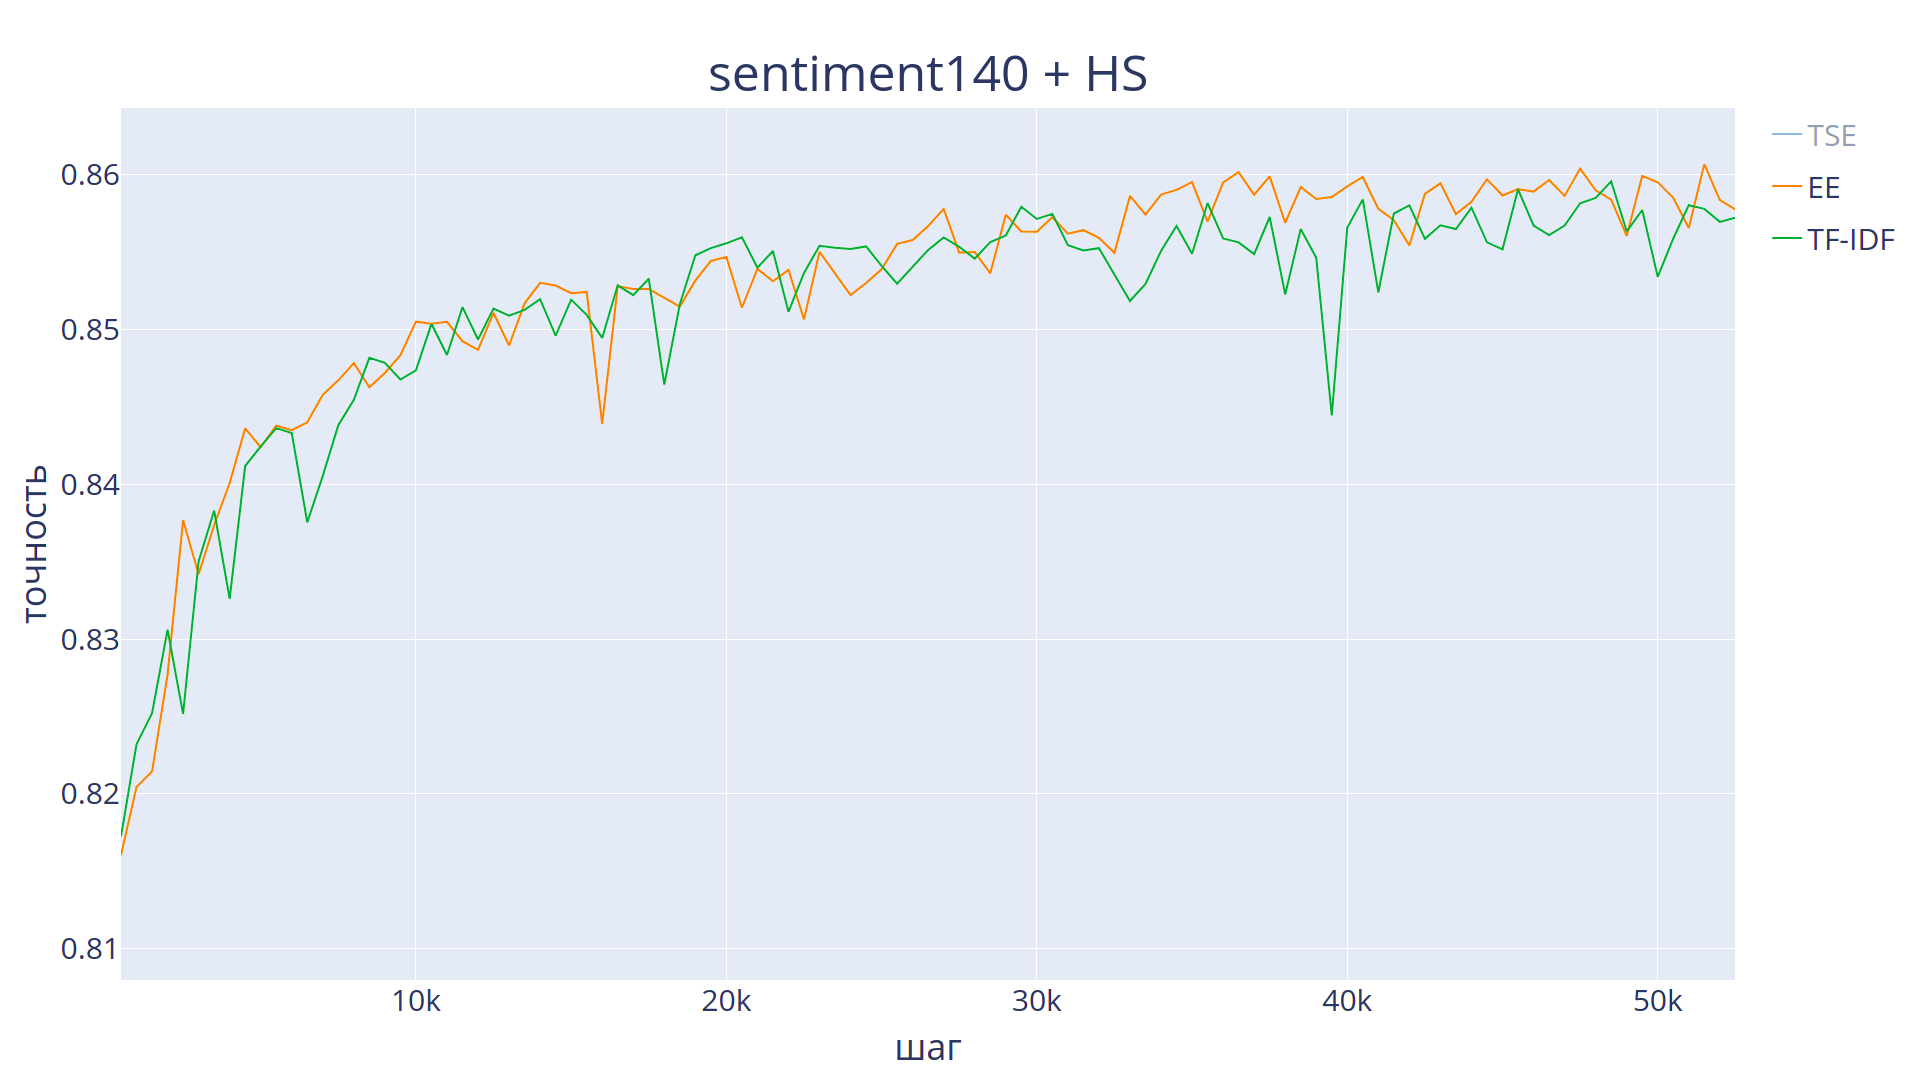
\includegraphics[scale=0.18]{s140_hyperbole}
	\end{center}
\end{frame}

\begin{frame}
	\frametitle{Влияние метрик на скорость обучения}
	TSE
	\begin{center}
		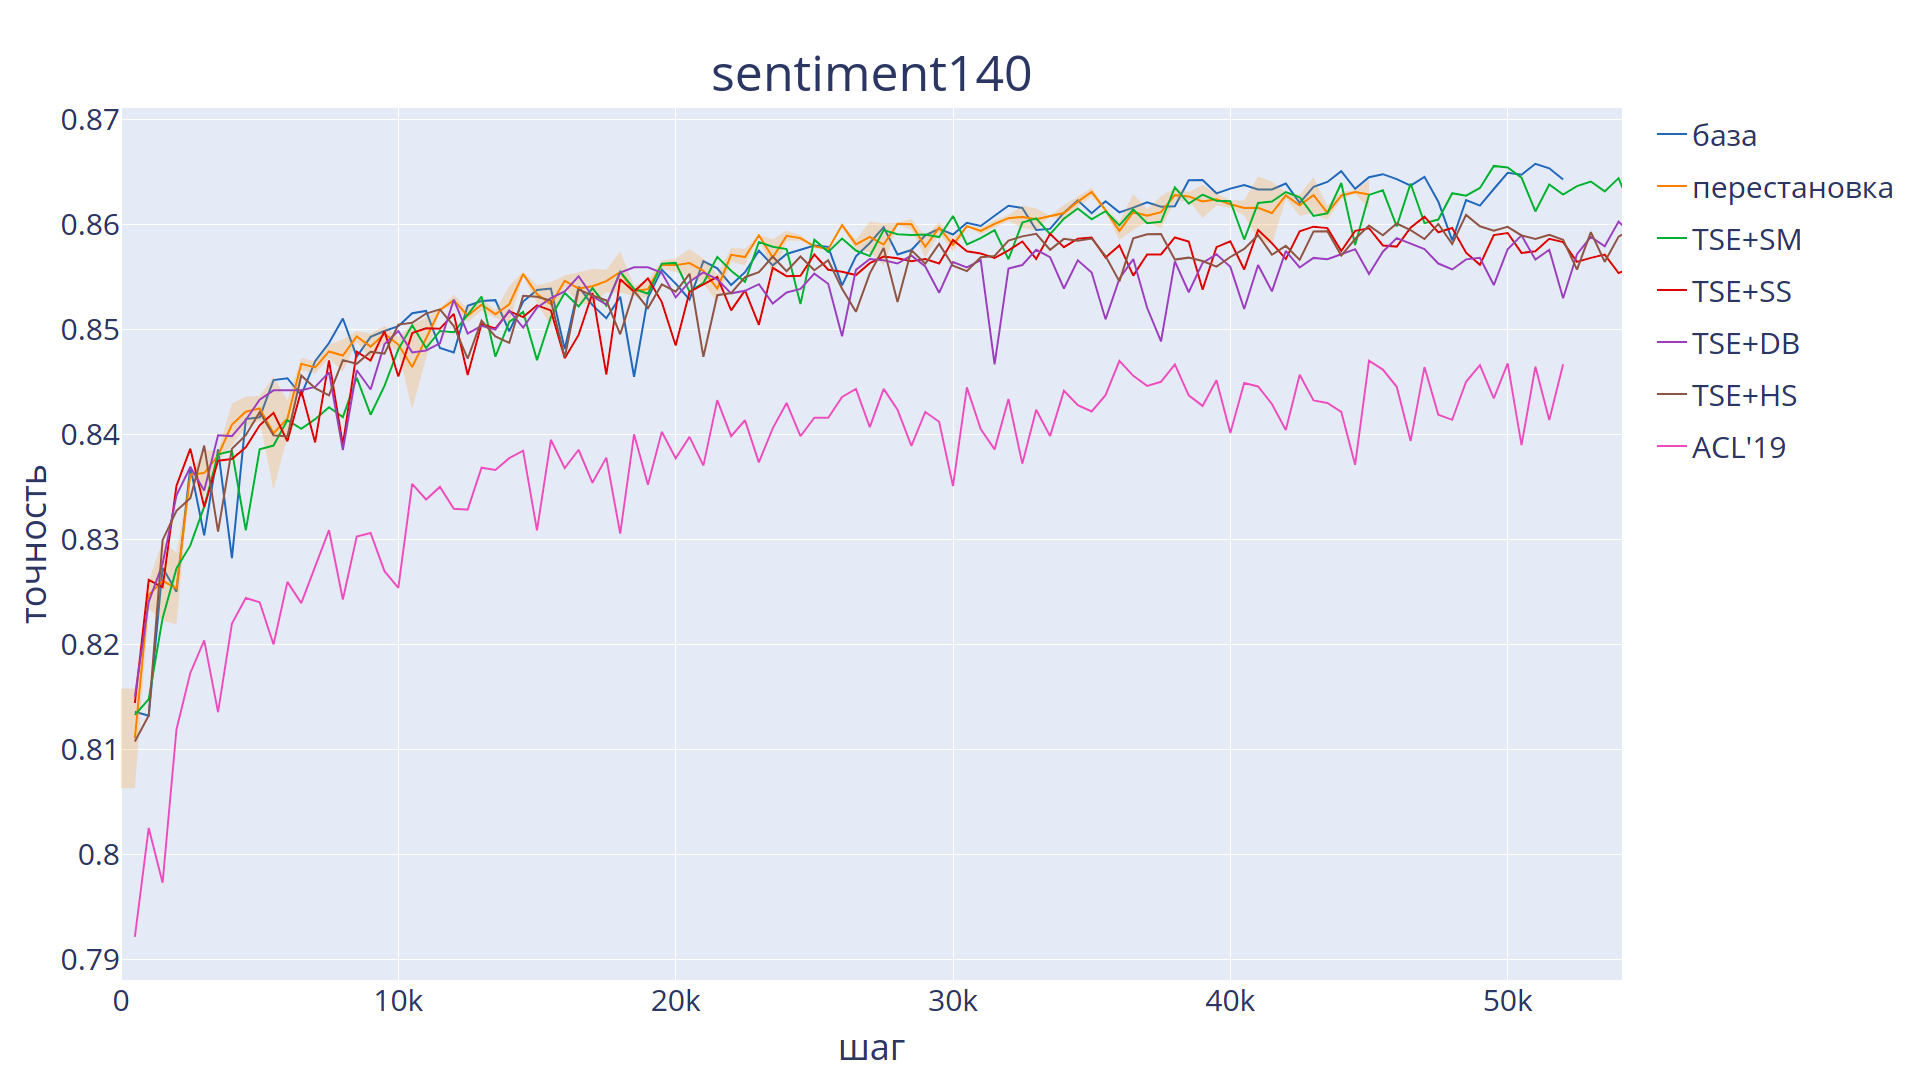
\includegraphics[scale=0.18]{s140_tse_final}
	\end{center}
\end{frame}

\begin{frame}
	\frametitle{Влияние метрик на скорость обучения}
	EE
	\begin{center}
		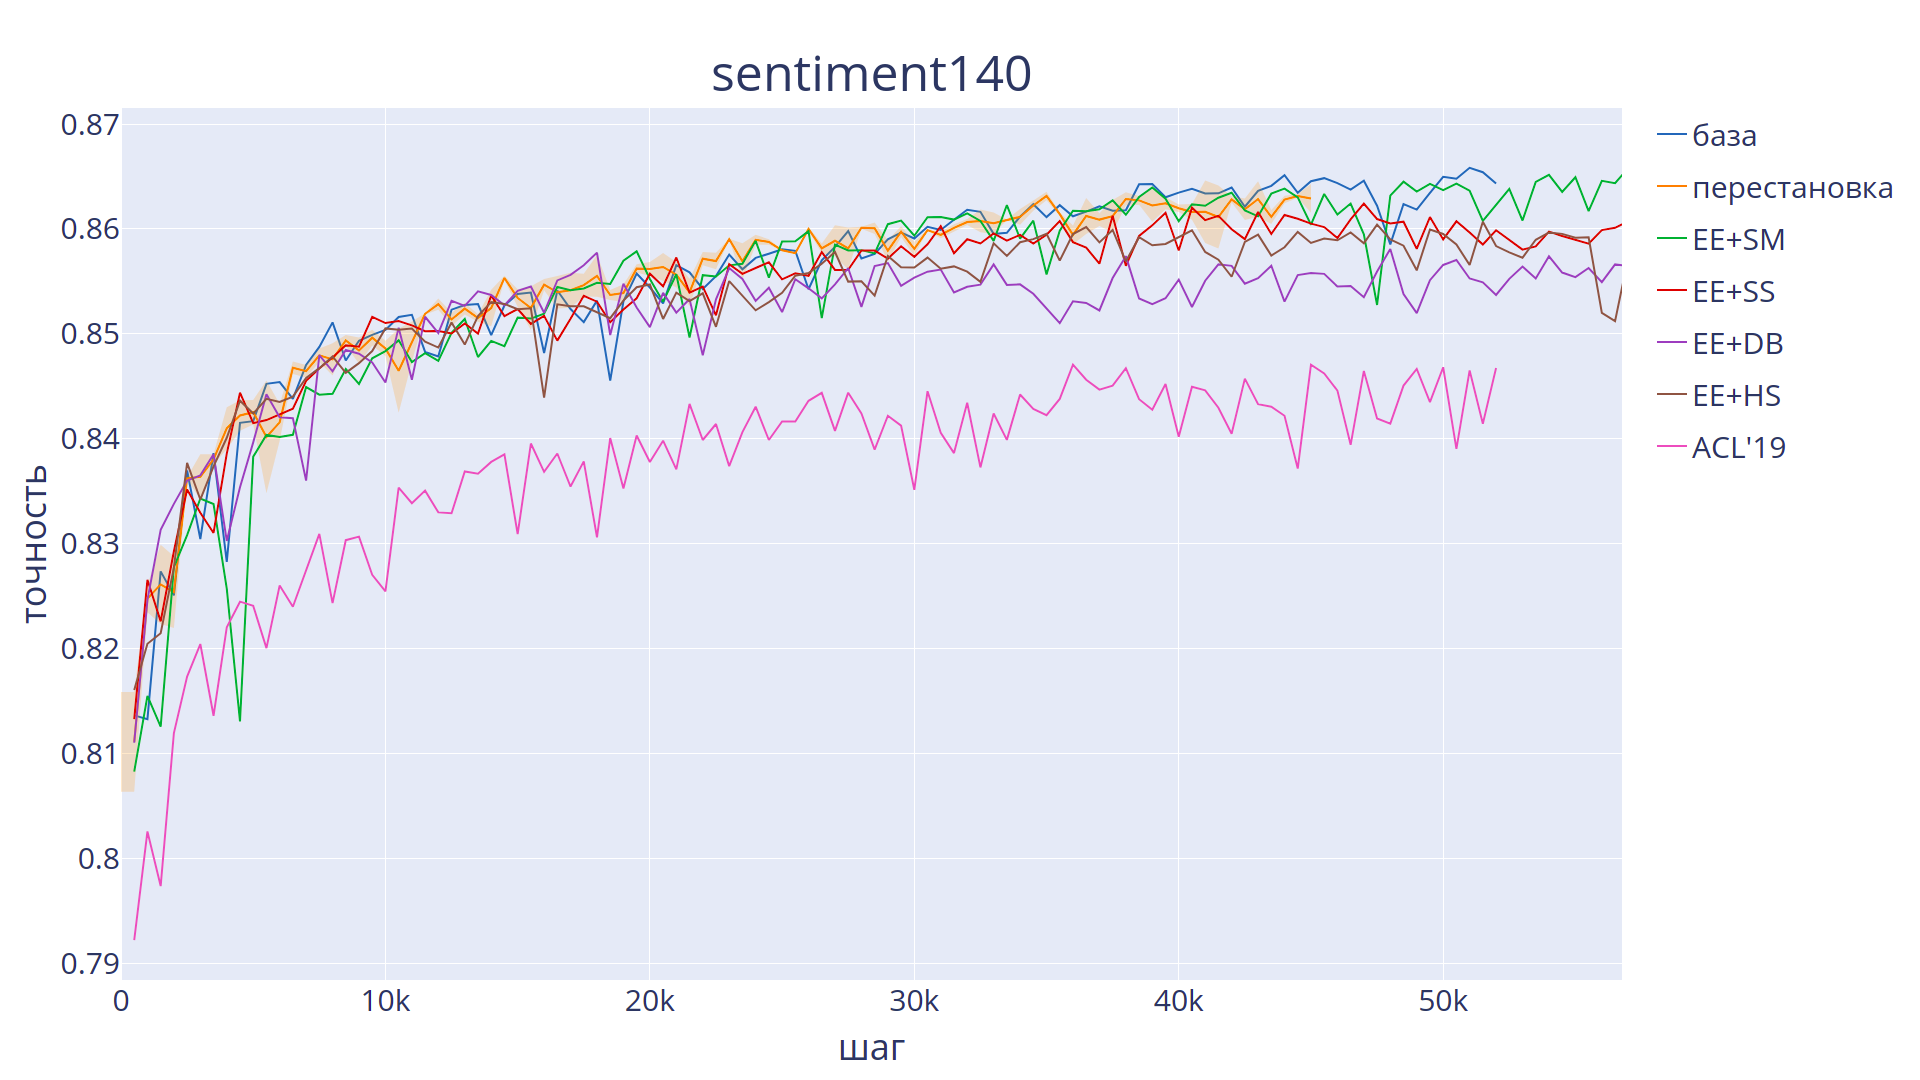
\includegraphics[scale=0.18]{s140_ee_final}
	\end{center}
\end{frame}

\begin{frame}
	\frametitle{Влияние метрик на скорость обучения}
	TF-IDF
	\begin{center}
		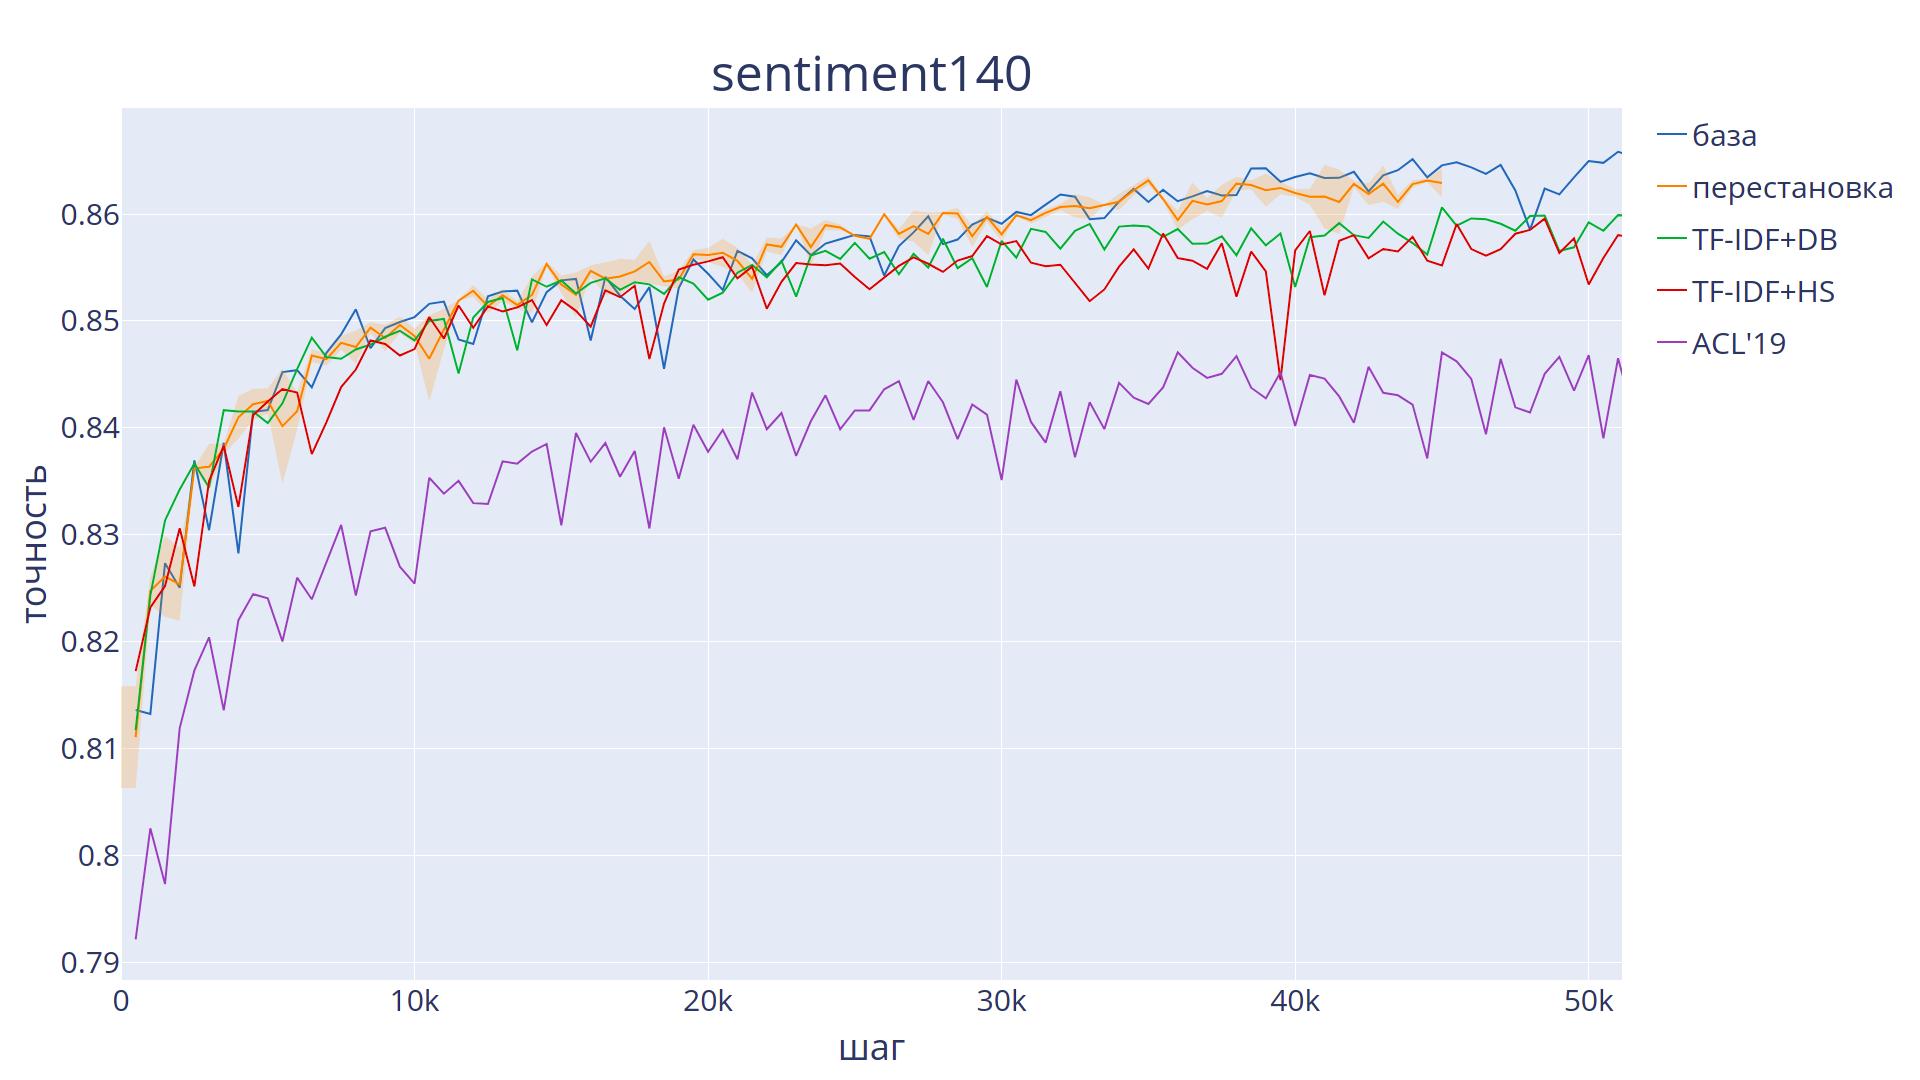
\includegraphics[scale=0.18]{s140_tf_idf_final}
	\end{center}
\end{frame}

\begin{frame}
	\frametitle{Результаты}
	\begin{enumerate}
		\item Найдены метрики оценки сложности текста
			\begin{itemize}
				\item метрики TSE и EE адаптированы под задачу обработки языка
				\item $(\text{TSE} \approx \text{EE}) > \text{TF-IDF} > \text{длина}$
			\end{itemize}
		\item Реализован механизм подсчета метрик на больших объемах данных
			\begin{itemize}
				\item Реализован механизм подсчета статистик для вычисления метрик
				\item Реализованы алгоритмы вычисления метрик
			\end{itemize}
		\item Проведено сравнительное исследование метрик
			\begin{itemize}
				\item задача классификации (sentiment140, HND)
				\item несколько семплеров
				\item Показано ускорение обучения относительно существующих результатов\footnote[1]{ACL'19}
			\end{itemize}
		\item Пока не удалось добиться существенного ускорения на задаче классификации относительно базового подхода
	\end{enumerate}
\end{frame}

\begin{frame}
	\frametitle{Дальнейший план работы}
	\begin{itemize}
		\item исследовать отношения метрик на задаче машинного перевода
		\item попытаться обобщить подход вычисления TSE и EE на большие $k$
		\item попытаться добиться ускорения на задаче классификации
	\end{itemize}
\end{frame}

\end{document}